\documentclass[letterpaper,10pt]{article}
\usepackage[margin=1.5in]{geometry}

\usepackage{epsfig,endnotes}
\usepackage[flushleft]{threeparttable}
\usepackage{amssymb}
\usepackage{graphicx}
\usepackage{amsmath}

\usepackage{url}

\newcommand{\keywords}[1]{\par\addvspace\baselineskip
\noindent\keywordname\enspace\ignorespaces#1}

\begin{document}

%don't want date printed
\date{}

\title{\Large \bf From Helios to Zeus}

% \author{Georgios Tsoukalas \qquad  Kostas Papadimitriou\\ 
% Panos Louridas \qquad Panayiotis Tsanakas\\[.5cm]
%  Greek Reseach and Education Network (GRNET),\\
% 56 Mesogeion Avenue, Athens, Greece\\
% \{gtsouk,kpap,louridas,tsanakas\}@grnet.gr}


\maketitle

% Use the following at camera-ready time to suppress page numbers.
% Comment it out when you first submit the paper for review.
\thispagestyle{empty}

\subsection*{Abstract}

We present Zeus, a verifiable internet ballot casting and counting
system based on Helios, in which encrypted votes are posted eponymously
to a server, then are anonymized via cryptographic mixing, and
finally are decrypted using multiple trustee keys. Zeus refines the
original Helios workflow to address a variety of practical issues, such
as usability, parallelization, varying election types, and tallying
through a separate computing system.
In rough numbers, in the first seven months of deployment, Zeus has been
used in more than 40 elections, tallying a total of more than 11000 votes.

\section{Introduction}

Helios~\cite{adida:2008} (\url{http://heliosvoting.org}) is a well
known system for internet voting, in which the entire process is
carried out through digital means---there is no paper trace, nor
ballots in physical form. Instead, there is a trail of mathematical
proofs linked together that can verify the correctness of every step
in the voting process. Helios has been used in several real world
elections and its basic architectural design has proven robust.

In the summer of 2012 our organization was asked to provide a system
for electronic voting to be used in elections in universities in
Greece. Based on its good track record and the body of work that had
been published on it, we decided to see whether Helios could fit our
needs. Unfortunately, we found that it could not, because of the
voting system that would be used in the elections we were called to
run.

We therefore had the problem of creating a system that could be used
for the required elections, scheduled to take place in approximately
three months time. Having no time to start from scratch, and having
no intention to re-invent the wheel or to embark on cryptography
research, we set out to develop a system based on Helios, as much as
possible, with the necessary modifications to suit our needs. The
system came to be known as Zeus (thus remaining in the pantheon of
Greek gods) and has been used with unequivocal success for many
elections over several months now. That was especially satisfying
since the use of Zeus was not without critics, for reasons that we
will explain below.

The contribution of this paper is not any new electronic voting
protocols or an entirely new voting workflow; we have adopted and used
proven systems and ideas that have already been described in the
literature. Our contribution is:
\begin{itemize}
\item An extension of an existing e-voting system, Helios, so as to be
  able any kind of voting systems, such as Single Transferable Vote.
\item A new use of audit votes, both as a means of checking the
  integrity of voting from the user's side, and as channel of
  authenticated communication with the user.
\item A description of a working e-voting system that has been used in
  many real-world elections, by not especially technically-savvy
  users.
\item An account of the experience of using an e-voting system in a
  particularly adversarial context, in over 40 real-world elections
  involving more than 11000 voters in total.
\item A description of the usability, accessibility, and logistical
  issues we had to tackle.
\item An outline of the internal design and implementation choices.
\end{itemize}

The rest of this paper proceeds as follows. 
In Section~\ref{sec:related},
we discuss related work and the roots of Zeus.
In Section~\ref{sec:challenges} we discuss Zeus's background and outline
the practical problems we faced and our approach to solve them.
In Section~\ref{sec:voting_overview} we offer an overview of the voting
process from the user's point of view.
In Section~\ref{sec:crypto_workflow} we go through the complete
cryptographic workflow elaborating on technical details and the
population of the \emph{poll document}, which contains all data
and proofs to verify the election.
In Section~\ref{sec:experience} we relate our experiences with the
deployment and use of Zeus as a service for elections over the internet.

\section{Related Work}
\label{sec:related}

Zeus is based on Helios~\cite{adida:2008}, an electronic voting system
developed by Ben Adida. The original Helios publication
\cite{adida:2008} proposed cryptographic mixing via
Sako-Kilian~\cite{sako:1995} / Benaloh~\cite{benaloh:2006}
mixnets~\cite{sako:1995} of ballots for their anonymization. Mixnets
were dropped in version 2 of Helios, which was used for elections at
the Universit\'{e} Catholique de Louvain in 2008, because in the
then-existing implementation they could not accommodate the need for
votes having different weights according to the voter's
category~\cite{adida:2009}. In place of mixnets homomorphic
tallying~\cite{cohen:1985} was adopted, as it was argued that it was
``easier to implement efficiently, and thus easier to
verify''~\cite{adida:2009}.

Homomorphic tallying operates directly on \emph{encrypted} votes,
tallying them all up in a single encrypted result, which is the only
piece of information that is decrypted. This is much easier
computationally but sacrifices generality because the tallying
algorithm must be encoded in the cryptographic processing itself---one
cannot get results in the form of individual ballots as they were
submitted.

On the other hand, mixing shuffles the set of votes in a provably
correct but practically untraceable way, therefore anonymizing it. The
output is the same set of unencrypted ballots as they were before
encryption and submission, only in random, unknowable order. Then any
method of tallying can be applied to compute results. Although Helios
itself is not using mixnets any more, a variant has been developed
that does~\cite{bulens:2011}; however the code is not publicly
available (nor was it available to us in any way).

From the voter's point of view, there has been a published usability
analysis of Helios~\cite{karayumak:2011}. From the elections we held
we have gathered our own experience on usability, and in fact the user
interface of Zeus is completely re-worked.

Over time researchers have explored possible vulnerabilities in
different versions of Helios~\cite{heiderich:2011}. To the best of our
knowledge these attacks are not applicable to Zeus.

More recently, the question of endowing Helios with everlasting
privacy has been explored~\cite{demirel:2012}. Helios's offers
computationally secure privacy, i.e., it is currently prohibitively
expensive, from a computational point of view, to break voter
anonymity. This does not preclude, however, that it will be
impractical in several years' time. Protocols for everlasting privacy
can be used for both homomorphic and mixnet-based elections. Zeus,
like Helios, relies on computational privacy and it would be possible
to explore the adoption of an everlasting privacy approach.

Due to the switch from homomorphic tallying to mixnets and other
requirements and refinements presented below, the Zeus software only
retains 50\% of the original source code, including the entire
homomorphic tallying support, which is unused.

\section{Zeus Background and Challenges}
\label{sec:challenges}

Zeus was initiated after the use of electronic voting was permitted by
decree for the election of the Governing Councils of Higher Education
Institutions in Greece. In each institution the Governing Council is
directly elected by its faculty and is its main governing body. The
election uses the Single Transferable Vote ({\sc stv}) system, in which
voters do not simply indicate the candidates of their preference, but
also rank them in order of preference. 

When we were charged with providing an implementation of a system
implementing electronic voting we decided to investigate Helios's
suitability, as we needed a mature system with a proven record in real
world elections and published open source code. The current version of
Helios (version 3) allows internet elections from end-to-end: from the
moment the voter casts a ballot through a web browser to the
publication of election results. It does that by never actually
decrypting the ballots but performing a series of homomorphic
calculations on them. In the end, the results of the calculations are
decrypted and published. 

Although using a single system for the whole process is appealing, the
use of homomorphic tallying in Helios cannot accommodate voting
systems in which not just the individual choices on the ballot matter,
but the whole ballot itself. In {\sc stv}, homomorphic tallying could pass
to the {\sc stv} algorithm the information that a certain candidate has been
selected in rank $r$ by $n$ voters, but this is not enough, as the whole
ballot and not just each rank separately is passed around during {\sc stv}'s
counting rounds.

We realized, however, that it is not necessary to use Helios's
homomorphic tallying capabilities. We decided to use Helios for
\emph{counting the ballots}, not for producing the election results.
Once we do have a verifiable ballots count, this can be fed to an STV
calculator, or indeed to a calculator of any voting system. Since the
ballots are published, and the algorithm is also published, a third
party can always verify that the results are correct.

\section{Overview of the Voting Process}
\label{sec:voting_overview}
% Merge this with workflow below

Each poll in Zeus comprises the following phases:
poll preparation, voting, processing, and tallying.

\subsection{Poll Preparation}
A Zeus account is created for the organizers of the poll.
Logging into the system with this account enables creation of new polls
through a submission form.
The account holder, that is the \emph{poll administrator},
sets the title, description, dates, and other information for the new
poll, and chooses who the trustees are going to be.
Next, they proceed to select the type of the election and define the
content of the poll accordingly.
Depending on the election type,
the content can typically be either a single list of candidates to rank,
or multiple party lists with candidates to select candidates from one,
or multiple questions for each to be answered by choosing one or more of
the provided answers; see Section~\ref{sec:ballot_encoding} 
and Section~\ref{sec:approval_counting} for details on the types of elections 
supported. Then, the administrator uploads the list of voters that may 
participate in the poll. A simple {\sc csv} format is used, easily 
exported from spreadsheets.

Before voting starts each of the trustees must visit Zeus's website
and generate and register their encryption keys for the poll.
The trustees do not need an account to enter the system.
Instead, upon their designation as trustees, Zeus sends them a
confidential invitation which they can use to log in to the system
and perform their duties.

Thus far, trustees are designated by their e-mail address, and the
invitation is sent via e-mail as a secret link to Zeus's website.
However, it is easy for Zeus to be adapted to use any system for
designation and notification of trustees. Indeed, an adaptation 
for notifications via mobile phones was actually implemented but
has not been used or streamlined within the software yet.

\subsubsection{Trustee Key Generation}
Trustees must follow their invitation and log in to generate their
key pair. The generation takes place entirely in the web browser,
assisted with randomness downloaded from the server itself, 
due to poor randomness in browsers, a practice inherited from Helios.
After key creation, the trustee is prompted to save their private key,
and when they acknowledge it has been saved, the public key is uploaded.
However, the key registration is not yet complete---trustees are
required to verify that they have indeed secured the key by
presenting it so that it can be compared to the one uploaded.

\subsubsection{Finalizing the Pool, and Inviting Voters}
The administrators may edit all aspects of the poll, up until they
decide to \emph{finalize} (or \emph{freeze}) the poll.
After that, only limited editing is possible, and most importantly,
all registered voters are sent their confidential invitations to vote.

As with trustees, voters do not need an account, but use the secret
information in their invitation.
Visiting Zeus through the invitation link will initially display
information about the poll along with contact details and voting dates.
Once the appointed voting time has come, the voting booth is
automatically enabled and visiting voters are transferred there directly.

\subsection{Voting}
The voting booth, once opened, operates entirely locally without
further interactions with the Zeus server or any other site.
The voter may even disconnect from the internet while inside the booth.
The booth appearance depends on the election type, and after vote
selection users are asked to review and confirm their choices.
After vote submission, a receipt (see Section~\ref{sec:receipts}) is
generated which can immediately be downloaded, but which is also sent
to them via e-mail.

During voting, administrators have access to aggregate and detailed
statistics for the ongoing election.

Section~\ref{sec:voting} elaborates on the technical issues.

\subsection{Processing and Tallying}
After the appointed end time, voting is automatically disabled.
However, administrators may choose to extend the voting to a new end
time and date, even after expiration.
For the poll to be finally closed,
the administrator has to explicitly select so.
Then, the first mixing by Zeus proceeds automatically.
Once the first mix is complete, additional mixes by external agents
may be added one by one using generated confidential links.
Zeus provides a command line toolkit that, among other things, can
perform mixing given these confidential links.

Finally, the administrator ends the mixing process,
and the trustees are notified again for the decryption process.
Each one visits the Zeus website through the invitation link they have
just received.
The mixed encrypted ballots are downloaded to their client browser,
and they are prompted to present their secret poll key.
When this is provided, the ballots are partially decrypted 
and the output is sent back to Zeus.

When all partial decryptions are available, they are combined to produce
the final anonymous and unencrypted ballots.
Depending on the poll type, the ballots are either sent into another
system for tallying and reporting the results (if the tallying
and results presentation algorithm is implemented externally, as was
the case in the majority of elections we have run),
or the ballots are tallied and reported on by Zeus itself.
After the results are available,
the administrator may download an archive with all generated proofs.

\section{Cryptographic Workflow}
\label{sec:crypto_workflow}
% what enters the doc and what does not

Zeus uses essentially the same cryptographic workflow as in Helios
\cite{adida:2008}.
In this section we contribute the organisation of the Helios workflow
around a logical document that contains every cryptographically
significant piece of data for a poll,
which can be stored in an interoperable textual canonical form.

The handling of this \emph{poll document} has been implemented
in a generic and standalone software module, which is then extended by
the web application and the user interface to create a usable voting system.

This core module implements all the required cryptographic functions and
validations. The web application extends the abstract workflow module
and builds a usable voting system upon a database
that handles authentication, election formulation, vote submission,
and trustee interactions for key setup and decryption.
The user interface offers access to the web application through
a web browser, and locally performs vote preparation and encryption,
as well as trustee key generation and (partial) ballot decryption.

\subsection{Poll Stages}
The abstract workflow represents each poll as a structured document
and defines five consecutive stages for it, from creation to completion.
At each stage more data are recorded into the document,
either coming from the outside, such as votes,
or as results of processing existing data, such as vote mixing,
or both, such as final ballots decryption.

Once recorded in the poll document, data are never modified,
and each stage is validated upon transition into the next one.

At the final stage,
the document represents a full account of a completed poll,
containing everything needed to verify the process,
from votes, to results, to proofs.

\subsubsection{Creating}
\label{sec:creating}

At this stage, candidates, voters, and trustees
are recorded into the document.
The candidate list is just an ordered list of unique candidate names,
which are otherwise not important and are not interpreted.
However, different types of elections put special structure
within the candidate list, which is used at tallying time
to verify and count the ballot,
as discussed in Section~\ref{sec:approval_counting}.

Voters are likewise represented by uninterpreted but unique names.
For each voter,
Zeus generates several random numbers, the \emph{voter codes}, that can
independently be used both for audit votes and voter authentication,
as discussed in Section~\ref{sec:audit_codes}.

For trustees, only their public key is recorded.
For each poll, and additionally to any external trustees,
Zeus always creates and registers a new trustee key for each poll.
As per the Helios workflow, this allows the service operator to
provide anonymity guarantees in addition to those provided by
the appointed committee of trustees.

\subsubsection{Voting}
\label{sec:voting}
When all intended trustees have been recorded,
the poll may transition to the \emph{voting} stage
by combining (by a multiplication)
the trustees' public keys into a single \emph{poll public key}
that the voters must use to encrypt their votes.
After the formulation of the poll public key,
no trustees, voters, or candidates can be modified.

For each submitted vote, Zeus generates a cryptographically signed
receipt for the voter.
With the receipt the voter can later prove that
his vote submission was acknowledged as successful,
perhaps in the context of an investigation for a complaint.
Receipts are detailed in Section~\ref{sec:receipts}.

Each voter may submit a vote multiple times.
Each time, the new vote replaces the old one,
and the new receipt explicitly states which vote it replaces.
No vote can be replaced more than once.

Apart from normal votes, voters may submit \emph{audit votes} to verify
that their local system really does submit the vote they choose,
and that it does not alter it in any way.
The process is detailed in Section~\ref{sec:audit_codes}.

\subsubsection{Mixing}
\label{sec:mixing}
After voting has ended, the poll is put into the \emph{mixing} stage,
where the encrypted ballots are anonymized.
Only the ballots eligible for counting are selected, by excluding
all audit votes, all replaced votes, and all votes by excluded voters.

Voter exclusion is a digital convenience owning to
the voter's identity still being known after voting has ended.
Anonymity is achieved at the end of the mixing stage,
and not at cast time as in traditional ballot box polls.
The poll's officials may choose to disqualify voters if
it is discovered that they were wrongly allowed to vote, or if
their conduct during the election was found in breach of rules.
Neither the disqualified voter nor their votes are deleted from 
the poll document. Instead, the voter is added into an exclusion 
list along with a statement justifying the decision to exclude them.

The eligible encrypted votes are first mixed by Zeus itself
by a Sako-Kilian mixnet.
The bulk of the computational work in mixing is to produce
enough rounds of the probabilistic proof.
The work is distributed to a group of parallel workers,
one round at a time. Our deployment used 128 rounds and 16 workers.
Verification of mixes is likewise parallel.

After the first mix is complete, additional mixes by external agents
may be verified and added in a strict order in the mix list, using
Zeus's command line utility.

\subsubsection{Decrypting}
\label{sec:decrypting}

After mixing is complete, the final mixed ballots are exported to
the trustees to be partially decrypted.
The resulting decryption factors are then verified and imported
into the poll document.
Zeus's own decryption factors are computed last.

\subsubsection{Finished}
\label{sec:finished}
In the transition to \emph{finished}, all decryption factors are
distributed in parallel workers to be verified and combined together
to yield the final decrypted ballots.
The decrypted ballots are recorded into the poll document,
and then the document is cast into a canonical representation in text.
This textual representation is hashed to obtain a cryptographically
secure identifier for it, which can be published and recorded
in the proceedings.

\subsection{Vote Submission Receipts}
\label{sec:receipts}
For each vote cast a receipt is generated and returned to the voter,
as well as registered in the poll document.
The receipt is a text file with simple structure listing cryptographic
information about the vote and poll.
The receipt text is signed with the Zeus's own trustee key for the
poll, practical because Zeus is a trustee for every poll
as described in Section~\ref{sec:creating}.
The ElGamal signature is according to \cite{schneier:1995}.

The receipt contains a unique identification of the cast vote,
the vote (if any) which it replaces, the cryptosystem used,
the poll's public key along with the public keys of all trustees,
the list of candidates, the cryptographic proof that it was a valid
encryption, and the signature itself.

Although private information such as user name, IPs, and times
are logged in the Zeus servers, they do not appear in the receipt,
because we need the entire poll document to be publishable if
the poll's authority decides so.

\subsection{Ranked Ballot Encoding}
\label{sec:ballot_encoding}
In Helios, ballots consist of answers to binary ``yes'' or ``no''
questions, framed in the appropriate way. For instance, a voter
indicates $k$ out of $n$ candidates on a ballot by selecting them, in
which case the answer ``Would you like X as a Y?'' gets a yes (1),
otherwise a no (0). In {\sc stv}, as in any system in which we would need
the whole ballot to be decrypted in the end, the ballot must be
encoded in some way. We encode each ballot as a integer by assigning a
unique number to each possible candidate selection and ranking. The
total number of possible ballots is $p _{n1} + p_{n2} + \cdots + p
_{nk}$, where $p_{nk}$ is the number of sequences of $k$ objects out
of $n$, that is $p_{nk} = n(n - 1)\cdots(n - k + 1)$\footnote{The
  number $p_{nk}$ is also written $n^{\underline{k}}$, or $(n)_k$,
  called ``Pochhammer's symbol''~\cite[p.\ 48]{graham:1994}. In closed
  form it is $p_{nk} = \sum_{k=0}^{n} (-1)^{n-k}\left\{n \atop
    k\right\}x^k$, where $\left\{n \atop k\right\}$ is the Stirling
  number of the first kind~\cite{weisstein:pochhammer}.}. As each
ballot is sent in encrypted form to the Zeus server, for its encoding
number $b$ we must have $b \in [0, 10^p]$, where $p$ is the order of
the group used in the ElGamal encryption scheme, so the encoding does
not present a practical limit in real elections (if it did, we could
always break the number in parts and send them separately).

The implementation of the encoding follows closely the mathematical
definition. We encode each ballot as an integer by enumerating the set
$\mathcal{E}$ of all possible ballots. We take $k$ choices out of $n$,
for $0\leq k \leq C$, where $C$ is the maximum choices allowed in the
ballots \footnote{$N=C$ for the elections we hosted}, and we then take
their $k!$ permutations. Summing it up, all the possible ballots are
\begin{equation}
\label{eq:max_encoded}
|\mathcal{E}| = \sum^{C}_{k=0}\binom{n}{k}k!
\end{equation}
When enumerating, we first count the smaller selections (i.e. take
\textit{zero} candidates, then \textit{one}, then \textit{two},
\ldots) so that for small numbers of choices the encoded ballot will
have a small value, thus saving valuable bit-space.\footnote{ For
  example, selecting up to all of 300 candidates needs 2043 bits,
  while selecting 10 out of 1000 candidates needs only 100 bits.}

% gtsouk: describe the exact encoding / decoding algorithm for the
% ballots. 

\subsection{Tallying Multi-Question Approval Polls}
\label{sec:approval_counting}
In Section~\ref{sec:ballot_encoding} we have established the encoding
used for ballots that select a subset of the candidates and ranks each
one in it, in a strict order.

Multi-question approval ballots, however, are different.
There is a number of questions separated into distinct groups,
and each question has a number of possible answers.
Each question can demand a minimum and a maximum number of answers
to be selected for a ballot to be valid.
The minimum can be zero, which means a ballot may select a question
without selecting any of its answers.
This is useful for party list elections, where you can vote for
a party list without having to vote for any of the candidates in it.
Only questions from the same group can be selected in the same ballot.
It is not allowed to select an answer without selecting the question
it belongs to.
Selecting no answer at all creates an empty ballot and a blank vote.

In order to encode this into an ElGamal plaintext we had two options;
either create a new encoding for multi-question approval ballots,
or translate the approval ballots into ranked ballots and use the
existing encoding.
Due to time constraints we used approval-to-ranking translation for
its simplicity and malleability, a solution that proved to be very
practical.

The translation works mainly by structuring the candidate names.
Each candidate name has two parts, the question and the answer.
All answers to the same question are required to occur together
on the candidate list.
The first candidate of a question is special,
and instead of an answer, the second part of its name contains
configuration information such as the minimum and maximum answers,
and the group it belongs to.
Selecting a questions is signified by selecting this candidate entry.
Question groups are identified by consecutive integers starting with 0.

Given this structure, each approval ballot can be represented by
correct choices among those entries, i.e. those that respect
grouping, minimum-maximum answers, etc.
The selections are also required to appear in a strictly ascending order
within the ranked ballots.

Note that this embedding of approval ballots within ranked ones is
only relevant at ballot preparation and ballot counting.
Between those two stages they are treated as ranked ballots.
The user interface will never produce an invalid ballot,
but Zeus will always validate them at counting time.
An invalid ballot is an alert, because it means there was either
an error in encoding, or someone has voted incorrectly without using
the official web interface.
Voting non-interactively via Zeus's programmatic web interface
should not pose any problem in itself,
but because the voter might get it wrong,
or might be executing an attack,
it is prudent to look into such incidents.

\subsection{Audit codes}
\label{sec:audit_codes}
Audit codes are random numbers generated by Zeus and sent to each voter.
The purpose of these codes is dual.
First, they can be used to submit audit votes to test that the local
system, mainly the web browser, faithfully submits the votes it is
being instructed to.
Secondly, and optionally, they can be used to authenticate voters in close
integration with audit votes.

Audit votes work by ruining the plans of an attacker who might otherwise
compromise the voter's computer and alter the voter's selections.
To ruin those plans one introduces uncertainty;
either the vote will be submitted normally and be counted,
or the vote will be revealed and published for all to see what it was.
If the attacker does not know what will be the fate of the vote,
they cannot decide whether to cheat or not.
If they cheat and the vote is published, they will be exposed.
If they don't and the vote is counted, they will fail.

Audit votes in Helios create this uncertainty by having the voter decide
on the fate of the vote, only \emph{after} it has been uploaded to the
server and therefore is made immune to the local attacker.
After submission of each vote, the voter is prompted to choose
between a normal vote and an audit one.

This is explicit and safe, but for Zeus it was deemed too dangerous to
\emph{require} all voters to make such a decision, because it would
require of all voters to understand what an audit vote does,
while a wrong button press, even accidentally,
would cause the true intended vote to be published.

In Zeus, a vote can be submitted either with an accompanying code,
or with no code at all.
Submissions without an accompanying code are accepted
as normal votes to be counted and no auditing is performed.
If a voter distrusts their local system and wishes to verify it
and submit their vote safely, then they should never submit
a vote without a code.

If a vote is submitted with an accompanying code, two things may happen.
If the code is \emph{not} among the ones the voter has received, then
the server considers it to be an audit.
If the code \emph{is} among those supplied by the server,
then it is cast as a normal vote.
Two different votes must never be submitted with the same code, because
the second time the attacker will know what to do.
This implies that the voter can only vote securely as many times as the
number of audit codes they receive.

The user interface of Zeus makes this process intentionally somewhat
obscure to the layman, so that its use without being certain what to
do is discouraged, but it is intended to be easy enough for those who
do understand: vote with a random ``wrong'' code many times and check
the audits, then vote with a ``correct'' and be done.

Therefore, Zeus makes auditing optional, by creating the required
uncertainty for auditing using the audit codes.
However, Zeus can be configured to \emph{require} a code with each vote
submission in which case the audit codes provide a secondary function
as an additional authentication factor.

This function is very useful because it helps combine a very convenient
but potentially insecure means, for example the e-mail,
with a quite secure and personalized one, for example the mobile phone.
Invitations, notifications, and descriptions relating to voting,
which can be voluminous texts with graphics,
can be sent by e-mail over the internet,
while the audit codes, which are conveniently small as a text,
can be sent to a mobile phone.
The voter would need both the e-mail and the mobile phone message in
order to vote successfully.

\subsection{Performance}
\label{sec:performance}
Mixing the votes both dominates the total processing time
and exponentiation dominates mixing calculations.
Python as a programming language has native support for arbitrarily
sized integers and exponentiation.
It is quite fast but we have used a high performing implementation
from\texttt{libgmp} via the \texttt{gmpy} python module.
This sped our exponentiations up about 7 times.
%We also noted that Python version 2.6 is significantly slower than
%version 2.7.

Still, the computational cost of mixing is so high that
it can only became practical when we parallelized it,
which is an algorithmically straightforward undertaking.

Zeus in its default 2048-bit cryptosystem with a 2047-bit order,
using 16 cores at 2.26 GHz can mix 10000 votes for 128 rounds,
a total of 12.8 million ciphers, in about 65 minutes
producing about 2 billion bytes of on-disk proof text data,
compressible to about half of it,
since numbers are in a hexadecimal canonical form and thus
2 bytes of text correspond to one byte of raw number data.

Although not trivial, this performance is practical enough that
we chose not to allocate more hardware so far,
our biggest election tallying about 1600 votes.

% \subsection{Cryptography and Proofs}
% \label{sec:proofs}
% Although we have retained significant portion of the web application in
% Helios 3 server software, we have almost entirely replaced the
% cryptographic primitives, since everything was tuned to homomorphic
% tallying, and thus useless to us---even the cryptosystem.
% Fortunately, this undertaking served us well later
% in our need to parallelize, and to software-engineer intensive
% control and validation over primitives over a known code base.
% 
% Zeus uses by default an Elgamal cryptosystem on the prime-order quadratic
% residue subgroup of a 2048-bit safe prime.
% Integers that are non-residues and therefore not within the ElGamal group
% are encoded into the group by mapping them to their opposite residue.
% 
% For reference, zeus software dependencies for cryptography are:
% Random number generation \emph{(Fortuna)}, primality testing
% \emph{(Miller-Rabin)} and modulo inversion from \texttt{PyCrypto}.
% Exponentiation from \texttt{libgmp} via \texttt{gmpy} (really faster
% than Python's builtin \texttt{pow}).
% We have implemented all other operations in native Python and the Python
% standard library, including hashing (SHA-1 and SHA-256),
% and a textual canonical form for structured objects,
% because JSON has no canonical form and was prohibitively slow.
% We have studied \texttt{Helios}, \texttt{PloneVoteCryptoLib},
% \texttt{PyCrypto} for our implementation. % citations ?

% \subsection{Vote preparation}
% \label{sec:vote_preparation}
% Don't forget about andomness from server.

% TODO: References to softwares
% signed canonical representation of proof data
% enumerated encoding: only valid votes are encoded (less than limit)
% redundant encoding: decoded vote is checked for canonical form.
% browser compatibility.

% \subsection{Cryptosystem}
% Zeus uses the ElGamal cryptosystem on the prime-order-$q$ subgroup
% $\mathcal{G}$ of the quadratic residues of a safe prime $p = 2q + 1$,
% such that
% $$m \in \mathcal{G} \longleftrightarrow \mathcal{L}(m) = m^q = 1 \mod p$$
% $\mathcal{L}$ being the \emph{Legendre} symbol.
% For reference, we reproduce all the primitives we use in a table.
% All base numbers are in $\mathcal{G}$, all exponents in $\mathbb{Z}^{*}_q$,
% and all operations are $\mod p$, unless explicitly noted.
% We group $x=a, y=b, \ldots$ as $(x,y,\ldots)\equiv(a,b,\ldots)$.

% \begin{tabular}{rl}
% \textbf{modulus}       \, & $p \equiv 3(\mod 4)$ \hfill\textit{\small(safe prime)}\\
% \textbf{generator}     \, & $g: g^q = 1$      \\
% \textbf{order}         \, & $q = (q-1)/2$\hfill\textit{\small(ElGamal group prime order)}\\
% \textbf{secret}        \, & $x$               \\
% \textbf{public}        \, & $y = g^x$         \\
% \textbf{committment}   \, & $t$               \\
% \textbf{challenge}     \, & $c$               \\
% \textbf{response}      \, & $f$     \hfill\textit{\small(from proof)} \\
% \textbf{\parbox{7em}
%     {\setlength{\baselineskip}{.85\baselineskip}
%      \raggedleft
%      group \\
%      encoding}}        \, & $T: x \mapsto \left\{
%                             \begin{matrix}  x &,&\quad x^q=1 \\
%                                            -x &,&\quad x^q\neq 1
%                             \end{matrix}\right.\quad
%                             T^{-1}: e \mapsto \left\{
%                             \begin{matrix}  e &,&\quad e \leq q \\
%                                            -e &,&\quad e > q \\
%                             \end{matrix}\right.
%                             $ \\
% \textbf{secret nonce}  \, & $r, w$  \hfill\textit{\small(in encryptions and proofs)} \\
% \textbf{ciphertext}    \, & $(a, b)\equiv(g^r, y^r m$)
%                                     \hfill\textit{\small(encryption)} \\
% \textbf{plaintext}     \, & $m = a^{-x}b$
%                                     \hfill\textit{\small(decryption)} \\
% \textbf{reencryption}  \, & $(a',b')\equiv(g^{r'}a, y^{r'}b)$ \\
% \textbf{hashing}       \, & $\mathcal{H}(n_0n_1n_2\ldots)$
%                             \hfill\textit{\small(hash textual representation of numbers)} \\
% \textbf{discrete log}  \, & $y = g^x \Rightarrow \log_gy=x \;\leadsto\;$
%                                     \textbf{\small prove you know} $x$ \\
%                        \, & $(t, c, f) \equiv (g^w, \mathcal{H}(t), w+xc)$
%                                     \hfill\textit{\small(prove knowledge)} \\
%                        \, & $g^f \overset{?}{=} ty^c$
%                                     \hfill\textit{\small(verify knowledge)} \\
%                        \, & $g, y, u, v \;\leadsto\;$
%                                     \textbf{\small prove} $\:log_gu = log_yv = w$
%                                     i.e. $(g, y, g^w, y^w)$ \\
%                        \, & $(t_g,t_y,c,f) \equiv (g^w, y^w, \mathcal{H}(t_gt_y), w+xc)$
%                                     \hfill\textit{\small(prove equality)} \\
%                        \, & $g^f \overset{?}{=} t_gu^c \wedge
%                              y^f \overset{?}{=} t_yv^c$
%                                     \hfill\textit{\small(verify equality)} \\
% \textbf{signature}     \, & $(z, s)\equiv\big(g^{w}, w^{-1}(m-zx)\mod (p-1)\big)
%                                     \quad w = 2w'-1,\: 3\leq w'\leq q$ \\
%                        \, & $m^s \overset{?}{=} y^zz^s$
%                                     \hfill\textit{\small(verify signature)} \\
% % TODO: cite Fiat-Shamir, Schnorr, Chaum-Pedersen, HAC in this table
% \end{tabular}

% \subsection{Creating}
% \subsection{Voting}
% \subsection{Mixing}
% \subsection{Decrypting}
% \subsection{Validation}

% \subsection{Election User Interface}
%
% The users of Zeus were not expected to be experts in cryptography, or
% to have any knowledge of computer science; we could only assume
% familiarity with internet browsing, since the electoral body comprises
% people with heterogeneous characteristics. A significant design goal
% was therefore \emph{interface}, and \emph{workflow} simplicity. At the
% same time, the knowledgeable voter needed access to all information
% and functions needed to both understand and verify the process.

% \subsection{Zeus Users}

% Zeus distinguishes the following classes of users:

% \begin{itemize}
% \item Election administrators
% \item Election committee members
% \item Voters
% \end{itemize}

% Election administrators are responsible for setting up an election;
% that is, starting a new election instance in Zeus, setting the date
% for the election, entering the particulars of the election committee
% members and the list of voters. During the election the administrators
% are responsible for updating the list of voters (i.e., adding,
% removing, or updating the details for a voter) and extending the poll
% times, if necessary. When polls close the administrators are
% responsible for starting the ballot mixing and vote count process.
% Election committee members hold the cryptographic keys for the
% election. Before the election starts they have to create their keys
% and upload the public parts to the Zeus server. During decryption each
% election committee member partially decrypts the ballots using the
% private part of the key. Voters visit the voting booth to cast their
% vote; they can vote repeatedly until polls close.

% Election administrators access Zeus through a username and password.
% Election committee members and voters access Zeus through URL links
% that are sent to them by the system, as we see below.

% \subsection{Administrator View}
% \subsection{Voting Booth}
% \subsection{Auditing}

% \section{Ballot Submission}

% The submitted ballot contains
% %gtsouk: describe the conntents of the submitted ballot
% A submitted ballot is a JSON object of the form:
% \begin{verbatim}
% {
%   answers : [];
%   election_hash : ;
%   election_uuid : ;
% }
% \end{verbatim}

% \section{Election Verification}

% %gtsouk: describe the election verification algorithm

% \section{Implementation Considerations}

\section{Experience}
\label{sec:experience}

To date, Zeus has been used in 45 elections around Greece.
Figure~\ref{fig:elections_to_date} shows the number of registered
voters and of those who actually voted in each election. The
registered voters in all elections totaled 14171, while the voters
that actually took part in the elections totaled 11133;
Figure~\ref{fig:elections_to_date_boxplot} shows a boxplot of
election numbers. Elections were carried out successfully in all
planned institutions. This was a significant success, as the stakes
were particularly high and the voting process charged with emotions.
To understand that it is necessary that we provide some surrounding
context.

\begin{figure}[ht]
  \begin{center}
    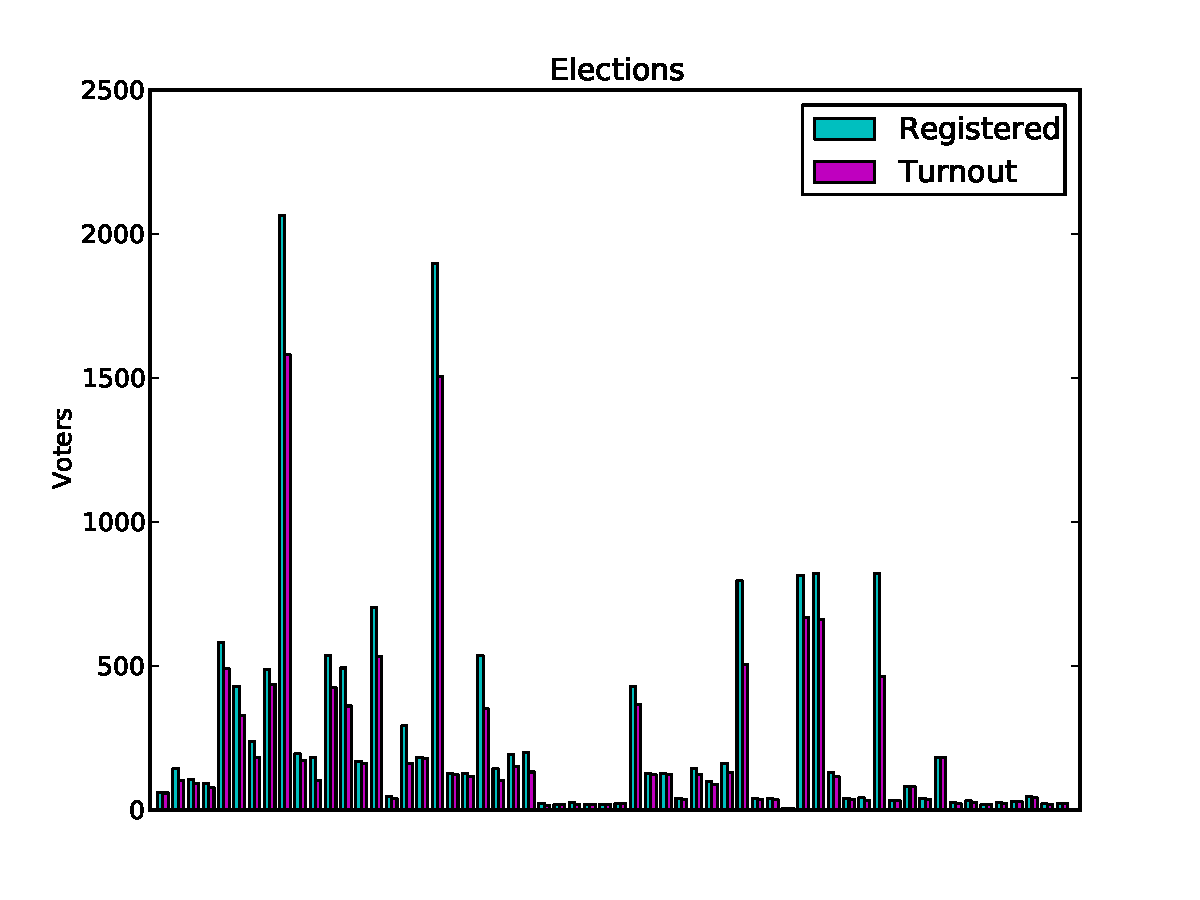
\includegraphics[scale=0.7]{elections_to_date.pdf}
  \end{center}
  \caption{Zeus held elections to date.}
  \label{fig:elections_to_date}
\end{figure}

\begin{figure}[ht]
  \begin{center}
    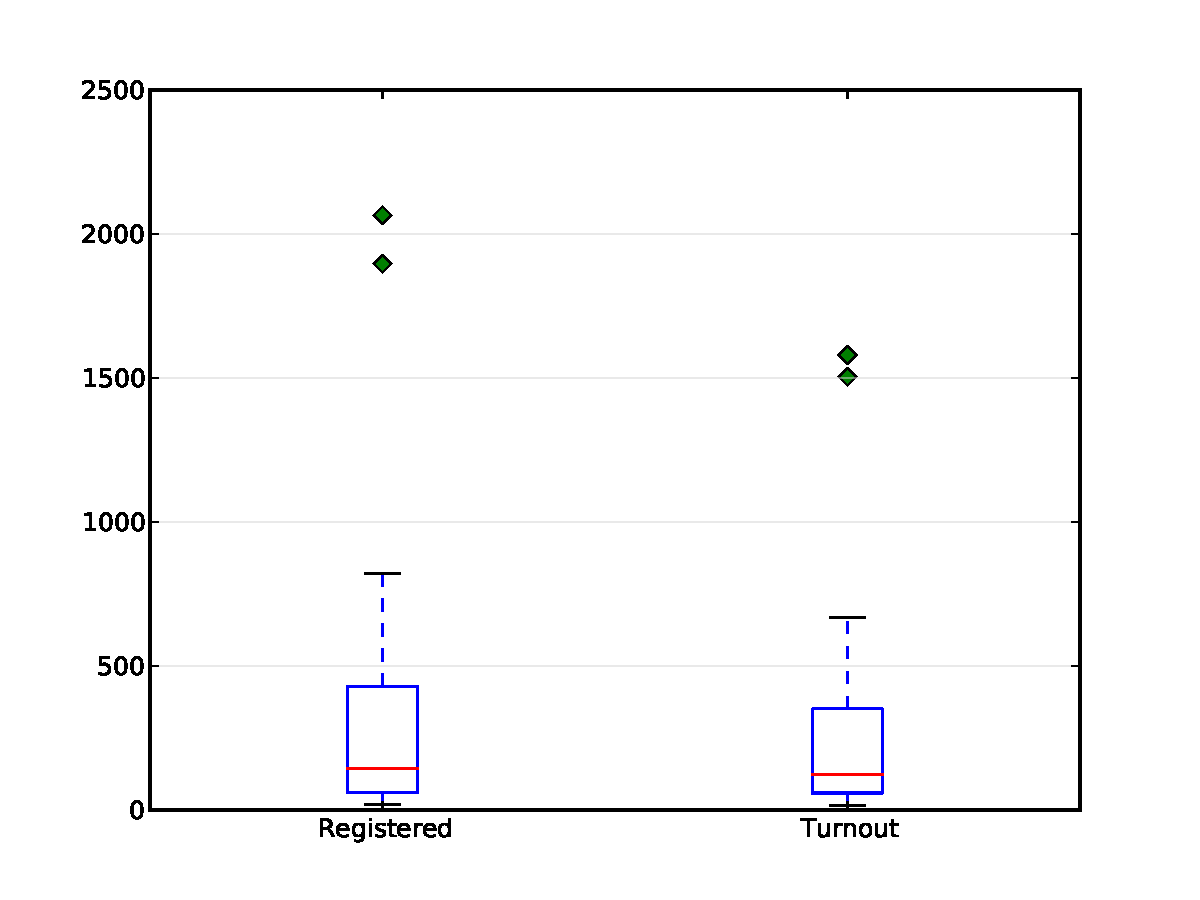
\includegraphics[scale=0.7]{elections_to_date_boxplot.pdf}
  \end{center}
  \caption{Boxplot of Zeus held elections to date, for registered
    voters and those who actually voted. Each box shows the upper and
    lower quartile with a line at the median. Whiskers show the values
    within 1.5 times the box quartiles.}
  \label{fig:elections_to_date_boxplot}
\end{figure}

The law that instituted the Governing Councils in Greek educational
institutions met resistance from some political parties, student and
academics unions. A widespread means of protest was to disrupt the
election of Governing Councils, so that they could not be selected.
Successive aborted elections pushed forward the adoption of electronic
voting, which then in brought Zeus into the controversy. 

In particular, the controversy meant that some political parties were
against the use of Zeus, or any form of electronic voting. As a
result, Zeus was the subject of a number of public denouncements and
letters, detailing weaknesses of electronic voting systems in general
and Helios in particular. These did not challenge Zeus, as the
weaknesses applied to older versions of Helios. Although Zeus was open
sourced from the start and we welcomed constructive criticism or the
exposure of unknown vulnerabilities, we did not receive any. The
atmosphere was at times vitriolic, as when a mainstream political
party called the people behind Zeus ``techno-fascists'', thus
introducing a new term in the greek lexicon and bemusing the people
involved in the whole effort.

This led to attacks on Zeus, and the voting process supported by Zeus.
None of them was eventually successful. We describe them briefly in
Section~\ref{ssec:attacks}. A discussion on other security-related
aspects follows in Section~\ref{ssec:security-discussion}. We round up
with a presentation of voting logistics in
Section~\ref{ssec:logistics}.

\subsection{Attacks}
\label{ssec:attacks}

\subsubsection{University of Thrace}

The elections at the University of Thrace had been planned for October
24, 2012. Due to a coding bug, the polls opened the at the time the
election was frozen, on October 22. This was discovered by some
voters, who went on to vote before the official poll opening. The
issue was publicized and the election was annulled and repeated at a
later date. Technically, the election could have proceeded without a
problem, since there was no way anybody could have tampered with the
election results, but the issue was sensitive and politicized, so that
the election committee took the most cautious route.

Elections were called again for October 29, 2012, with polls opening
at 9:00. At dawn our Networks Operations Center noticed a large number
of connections to Zeus. Upon investigation, it was found that Zeus was
the subject of a slowloris attack~\cite{slowloris}. The attach was
swiftly dealt with, and apart from some initial inconvenience did not
cause any real problems. Moreover, the attackers used static IP
addresses and could easily be traced and blocked.

\subsubsection{University of the Aegean}

The University of the Aegean had planned its elections for November 2,
2012. After freezing the election, and when the notifications to the
voters had been sent, voters started receiving additional
notifications containing bogus {\sc url}s from a cracked university server.
Although the bogus {\sc url}s were not functional, a number of users were
confused. The electoral committee decided to cancel the elections and
call new elections at a later date. To avoid similar situations in
coming elections we recommended the use of Sender Policy Framework
({\sc spf})~\cite{rfc4408} to institutions that had not been using it.

The repeat elections were held on November 9, 2012. The authorities at
the university had authorized the set up of a new mail server, to be
used solely for the elections, in which all voters were opened
accounts. The mail server was hosted outside the university's
premises. This avoided a problem that would have risen from a sit-in
at the building housing the main mail server, which had been switched
off by protesters at election day.

\subsubsection{Agricultural University of Athens}

On election day, November 5, 2012, protesters staged a sit-in at the
mail server building of the Agricultural University of Athens. The
mail server was switched off, cutting off access to e-mail, and
depriving voters that had not downloaded the access link from voting.
The university authorities responded by asking voters to come
physically to a location outside the campus, where they could be
issued with a new {\sc url}.

\subsubsection{University of Patras}

The University of Patras held its elections on November 7, 2012. Just
prior to the opening of the polls a slowloris attack was noticed and
dealt with.

\subsubsection{University of Athens}

A little while after polls opened at the University of Athens, on
November 12, 2012, protesters staged a sit-in at the university's
Network Operations Server and cut off internet access. This took
offline mail access to members of the university and, like in the
Agricultural University of Athens, deprived voters that had not
downloaded the access link from voting. More dramatically, the
internet shutdown affected all sorts of university services, including
internet connectivity to university hospitals.

The university responded by extending polling by three days. At the
same time, an alternative voter's notification scheme was implemented,
via which the voters would receive instructions for voting via {\sc sms}.
The sit-in was lifted on the last election day, as it was realized
that the elections would go on regardless.

\subsubsection{National Technical University of Athens}

A sit-in similar to the one at the University of Athens was planned at
the National Technical University of Athens. However, it did not last
long, as the {\sc sms}-based infrastructure was already in place, so
that it would be irrelevant, and the university authorities made it
clear that they would not tolerate the disruption. The election took
place without problems on December 10, 2012.

A different, more insidious kind of attack was revealed later on. A
few days before the election, one voter had contacted us complaining
that the link he had received did not seem to be functioning at all
(it should link to a page notifying the user about the coming
elections; instead, the user was redirected to the main Zeus page).
Two days before the election it was discovered that the user's e-mail
stored in Zeus had been changed, and a new e-mail had been sent to the
newly entered mail address. The user complained that he never used
that address, so another {\sc url} was issued and sent to his institutional
mail address. The voter voted without a problem on election day.

A few days afterwards a protesters' site announced they had
circumvented Zeus security by taking hold of a voter's {\sc url} after
contacting the election committee and asking them to update the
voter's contact details. That explained the e-mail change, and it
meant that it was the result of a social engineering attack. Luckily,
it had been caught in time---something the protesters did not let on.


\subsubsection{Recreate Greece}

Encouraged by the success of Zeus in previous elections, a new
political party, ``Recreate Greece'' (``dimiourgia, xana!'' in Greek)
approached us and enquired whether they could use Zeus for the
elections leading to, and during, their party congress. Although not
among our target constituency, we decided to allow the use of Zeus in
a ``best-effort'' basis from our part, since that entailed the
development of new, interesting functionality---specifically, party
list elections, elections with multiple questions and answers, and
elections where blank votes are not allowed.

It turned out that in one of their elections a voter wanted to show
that e-voting cannot be trusted since anybody can vote with a voter's
access credentials, if these are leaked. On April 6, 2013, the voter
posted his voter {\sc url} on a Facebook page. The electoral committee noted
the incident, and therefore moved to disqualify the ballots cast under
that voter's name. 

\subsection{General Security Issues}
\label{ssec:security-discussion}

As explained above, Zeus was born in controversy, and its use was
accompanied by much nay-saying. An important argument against the
system was that we were not to be trusted. After all, to the voters,
as well as to each election committee, Zeus is a black box running in
some remote virtual machine. It could be that we were really running a
show: instead of Zeus, voters were interacting with something else, and
we were putting on a pretense of anonymity and security. 

As we were not aware of a practical method to verify the integrity of
a running virtual machine, doubters were presented with two choices:
either they would have to take us on our word that we were indeed
honest, or they could download the code and run it themselves. Nobody
took the second option. 

Still, at several times throughout different elections we became aware
that people did not really believe us in our assertions that we were
honest and that the system behaved as we had argued it would. In two
distinct occasions members of the election committee discovered that
their election key could not be read by Zeus---a bad file. We had
instructed them to keep two copies on two different {\sc usb} sticks.
Luckily, in both instances the back-ups were readable. People, though,
were to various degrees sure that somehow we would be able to ``do
something'' about it, disregarding our assurances that the only thing
we could really do would be to re-run the elections from the beginning.

A similar veil of doubt appeared when people called us condidentially
during elections, and shortly after the ballot box had been closed, to
ask us ``how things were going'', and whether we had an indication of
the results. We were at pains to explain that there is no way we could
have such knowledge.

Doubt in whether Zeus does indeed what is purported to do manifested
itself also in a request we received twice to provide to the election
committee a log of the exact times each voter had cast a ballot. We
explained to the election committee that if the issue at hand was to
verify that all votes had been counted correctly, the correct
procedure was other, and that the requested information could in fact
be damaging in enabling fine-tuned attacks on privacy (an attacher
would check that a voter who had been coerced to vote did not vote
again afterwards). 

Zeus gives to the election committee a full set of cryptographic
proofs that can be used to verify the results. We had stressed that
these proofs would be the sole arbitrer of any dispute, and the only
material that could be really trusted. At some point in the elections,
though, we decided to provide, just for convenience, a {\sc pdf}
summary output of the results. We found out to our chagrin that a
plain, unsigned {\sc pdf} document carries more weight than any of our
pronouncements.

In particular, we used ReportLab's open source libraries for {\sc pdf}
creation (\url{http://www.reportlab.com/software/opensource/}). In one
election (elections for president of the Piraeus Technical Educational
Institute, held on March 26, 2013), a disgruntled candidate complained
to the election committee that the {\sc pdf} results' creation date
was before the ballot closing time. It turned out that he was right, and
that this was due to a bug with the {\sc pdf} libraries (which we
reported to ReportLab). The fact that we never meant the {\sc pdf}
document to be the definitive results record of an election seemed to
matter little. The issue was resolved after we issued an official
explanation, complete with details of the bug and possible fixes. The
authority of the {\sc pdf} document is something we came up against
repeatedly: people did not seem to care for any other kind of
authority apart from that given by the printed matter.

Regarding usability, we did not receive any particular complains from
the voters, except for one: that the system would not work with
Internet Explorer. The users were informed of that in the
notifications they received, but apparently not all of them noticed
it, or knew exactly how to download and install one of the supported
browsers (recent editions of Firefox, Chrome). The problem was pointed
out to them when they contacted the respective election committee
about their difficulties with and was thereby resolved; we did receive
an angry e-mail, though, from a voter who felt snubbed that she had
to go through such an ordeal. At the other end of the spectrum we saw
in an interview a mention of a voter who had voted in an airplane and
was very happy for it.

Voters were not expected to be knowledgeable about cryptography, and
we took care to smooth the use of Zeus for them. A lack of
understanding led to a few interesting interactions, with some voters
trying to read and understand their voting receipts---although the
e-mail attachments that contained them did not have a text suffix in
order to discourage careless handling of them. They then inquired why
they could not understand the receipt contents, and how they could be
sure that it was a valid one. This is something that could be solved
in time with better informational material and voter education on the
basic premises of the system.

In the same vein, nobody bothered to use the audit vote feature,
whereby a voter tests that their browser is not compromised. A few
asked about it, and when they understood what it was about decided it
was not worth the trouble. In truth, the voters that asked about it
found it confusing, and we had to visually downplay the related user
interface elements in order not to confuse the electorate.

Finally, nobody bothered to use our support for external mixnets,
although we did explain to those who asked that this was the only way
to guarantee anonymity if they could not trust us.

\subsection{Logistics}
\label{ssec:logistics}

Zeus is offered as a hosted service; hosting here entails more than
just a well-endowed virtual machine. Elections are a sensitive matter,
since people exercise their basic democratic right. They must feel
secure, and they must feel they are not slighted by their lack of
technical knowledge.

In every Zeus election we have a helpdesk of three persons involved
part time (and not all of the concurrently) before the election
starts, during the election itself, and after the ballot box closes.

Before the election started the helpdesk is tasked with helping the
election committee setting up the election. Although we have produced
manuals, for both the election committee and voters, people frequently
requested more engagement from our part. As an aside, we should point
out that {\sc rtfm} rules, as always, and the more so the more
technical a user is. We found that users with no particular computing
experience were more careful in their use of the system and more
conscientious in their use of the manuals provided, than users who,
emboldened by their prowess in computing, went on without bothering to
consult the documentation.

Our helpdesk colleagues help the election committee to generate
their keys and to set up the voters list, ensuring that the input
file, a simple {\sc csv} document, was well formed---not a trivial
matter, as it turned out, as despite our detailed instructions college
registrars often failed to produce an up to date list of eligible
voters with their current e-mails, or to create a spreadsheet with the
required columns. Once the e-mails containing the
voters links are sent the helpdesk handles bounces. The bounces
are forwarded to the election committee with the voter links removed,
so that the election committee can contact the voters and correct
their e-mail addresses but cannot abuse the system and start voting in
their stead. 

It could be possible, in this setting, for the administrators of Zeus
not to forward the bounces and to therefore compromise the system by
doing the voting themselves. This, though, would require of us to know
in advance which voters would not bother to contact the election
committee inquiring why they have not received their voter links, at
which point the election committee would discover that somebody else
has been voting for them. Even if we were crooks we would not run a
risk as high as this one.

During the election the helpdesk guides the election committee when
they are in doubt about how to correct a voter's details. This happens
when a voter contacts the election committee asking them to change
their e-mail address to another one. Then, at the end of each election
process, the helpdesk is sometimes asked to show the steps for the
mixing and decryption process, as well as the presentation of the
actual results.

In general, even though the helpdesk workload is not particularly
high, it has special time requirements, such as working out of normal
business hours to ensure that the communication with the election
committee and the voters is as prompt as possible. Both election
committees and voters can get very anxious when things are not working
in the way they may have anticipated.

% gtsouk: Including timing measurements, especially wrt differen versions of
% Python, GMP, etc.

% gtsouk: also instances where existing implementations were not up to
% par from a cryptographic point of view

\section{Discussion}

Zeus was a success beyond our expectations. It carried out all the
elections we were called to run by law. People must have been
reasonably happy with it, since following our official mandate we were
asked, and we continue to be asked, to help organize other elections
around the country: appointment of representatives for university
teachers' union congress, various elections for the selection of
rectors, deans, and department presidents, congress election for a
political party. We understand that the practical advantages of
e-voting outweighs any reservations the corresponding constituencies
may have. In a telling interchange, a member of an election committee
expressed his gratitude in high spirits, mentioning that in previous
elections they would have to spend the night counting, re-counting,
and dealing with possible complaints---while with Zeus they packed up
early in the evening.

We are continuing to maintain and improve Zeus in various ways, mainly
in allowing more kinds of elections with different ballot
configurations and improving usability based on the feedback we
receive. Zeus mixing is embarrassingly parallel, so we can easily scale
it up to bigger elections; decryption from the part of the election
committee however takes place on a local computer and may be limited
by the resources there. We are exploring way in which we could improve
performance, for instance, by developing and distributing a native
application.

At the time of this writing Zeus is actively used, and new elections
are announced that are using it. 

\section{Availability}

Zeus is open software, available at \url{XXX} (URL withheld according
to paper submission guidelines).

\section{Acknowledgments}

We would like to thank Professor Aggelos Kiayias for the interesting
discussions we had in the start of the project.

{\footnotesize
\bibliographystyle{acm}
\bibliography{zeus}
}


\end{document}

